%\documentclass{neu_handout}
\documentclass[a4paper, 10pt]{article}

\usepackage{url}
\usepackage{amssymb}
\usepackage{hyperref}
\usepackage{enumitem}
\usepackage{graphicx}
\usepackage{subfig}
\usepackage{caption}

\usepackage{floatrow}


\usepackage{comment}  
\usepackage{fullpage} % changes the margin
\usepackage[margin=0.45in]{geometry}
\pagenumbering{gobble}          
\usepackage{hyperref}

\begin{document}


\title{DS5230 Project Update 1 : Pattern Recognition in Accidents in the UK}


\author{
  Sahasrabhojanee, Adwait\ \\     \texttt{sahasrabhojanee.a@husky.neu.edu}
  \and
  Sreekumar, Sreejith\  \\ \texttt{sreekumar.s@husky.neu.edu}
  \and
  Yu, Xue \\  \texttt{yu.xue1@husky.neu.edu}
  \and
  Li, Xuexian  \\ \texttt{li.xuex@husky.neu.edu}
}
\maketitle
\section{Introduction}
The Department of Transport in the United Kingdom has extensively recorded all the road accidents over the years. Their records provide a comprehensive dataset to
explore the patterns in road accidents and identify factors that add to their causality. \\
  As an initial study of the dataset, we explore noticable patterns using statistical methods and exploratory data analysis. 

\section{Exploring accidents the UK region for trends and patterns }

\subsection{Spatial Study}  
The dataset comprises of accidents from England, Scotland and Wales. Making use of GPS data in the records, we isolated the top 200 cities/ suburbs where most number of
accidents have happened and geo tagged them. \\
    \begin{center}
      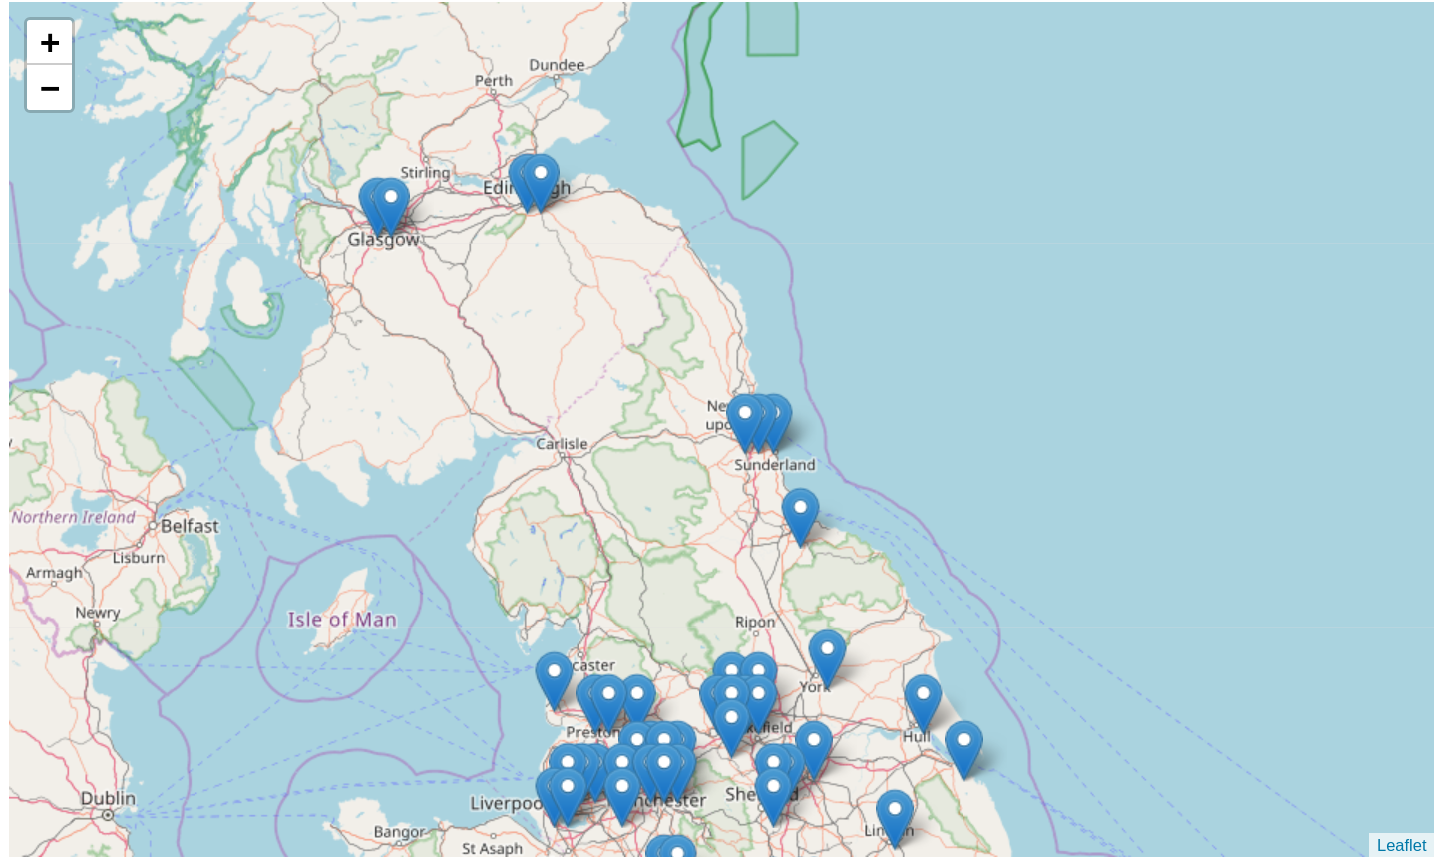
\includegraphics[width=70cm,height=6cm, scale=0.4,keepaspectratio]{map1.png}
    \end{center}

    \begin{center}
      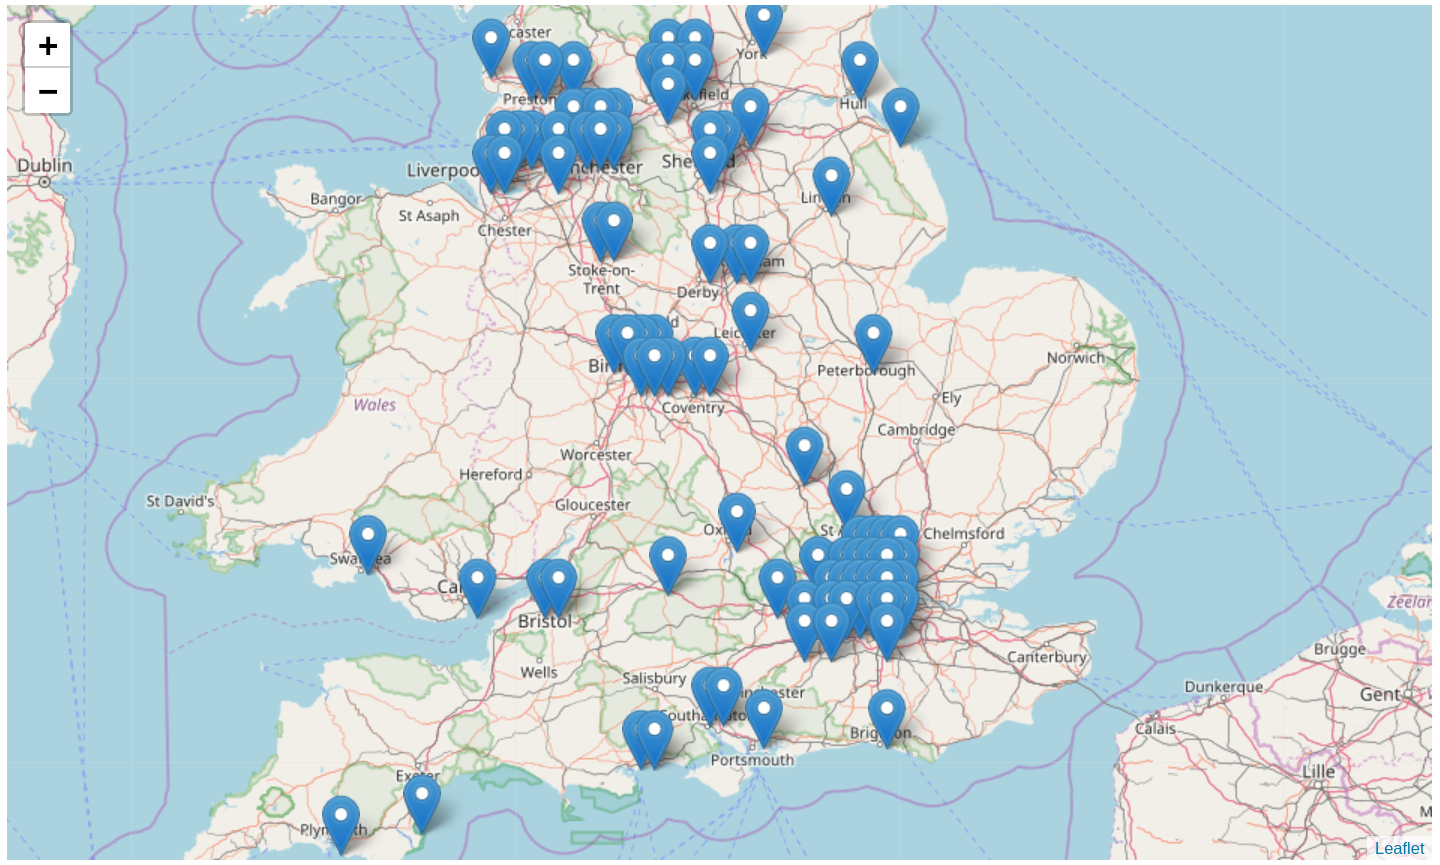
\includegraphics[width=70cm,height=6cm, scale=0.4,keepaspectratio]{map2.png}
    \end{center}

    Over the years from 2009-2014, the cities which stayed top 13 in the number of accident casualties are London, Birmingham, Kirklees, Liverpool, Leeds, City of Edinburgh, Wakefield, Rushcliffe, Sunderland, North East Derbyshire, Elmbridge, East Lindsey, and Manchester. As, we can see, there is a high concentration of pins around these areas. Unsurprisingly, these are the most populated cities in the UK[1]. \\

 We plotted a heat map showing the frequency of vehicles in different counties in the UK. The locations with high concentration of vehicles are more or less the same as the ones where the accidents are the highest. \\

 \begin{figure}
   \begin{center}
     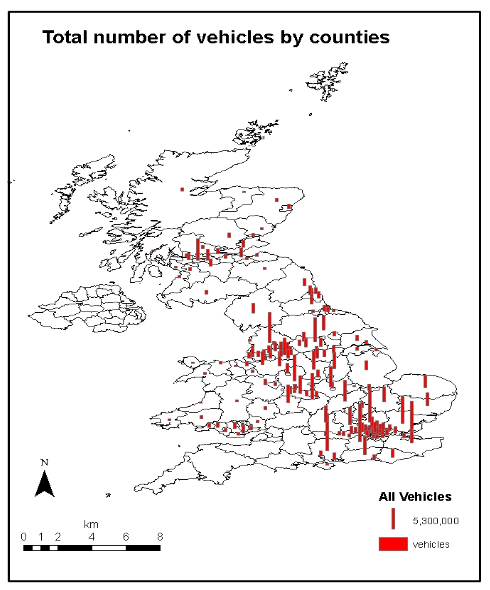
\includegraphics[width=70cm,height=6cm, scale=0.4,keepaspectratio]{vehicles-by-county.png}
     \caption{Total number of vehicles in various counties of U.K.(2014)}
    \end{center}
  \end{figure}

\subsection{Summary Statistics}
  Looking at the summary statistics of the records, we have: \\

  \begin{center}
 \begin{tabular}{|c c c c c|} 
 \hline
 Feature & Mean & Standard Deviation & Median & Mode \\ 
 \hline\hline\hline
 Police Force & 29.59 & 25.49 & 23 & 1  \\ 
 \hline
 Number of Vehicles & 1.826 & 0.709 & 2 & 2 \\
 \hline
 Number of Casualties & 1.34 & .82 & 1 & 1 \\
 \hline
 Speed Limit & 38.52 & 13.9 & 30 & 30 \\
 \hline\hline
\end{tabular}
\end{center}

  It is seen that most accidents are between two vehicles or between a vehicle and a pedestrian. Mostly, 1 casualty occurs in an accident.

    The dataset groups the severity of the accidents in levels 1-3. However, it's not mentioned which is more severe on this scale. Since understanding this is critical to our analysis, we mapped the proportion of accidents in each severity level with the number of officers police force who attended the scene, and the number of casualties. \\

   \begin{center}
     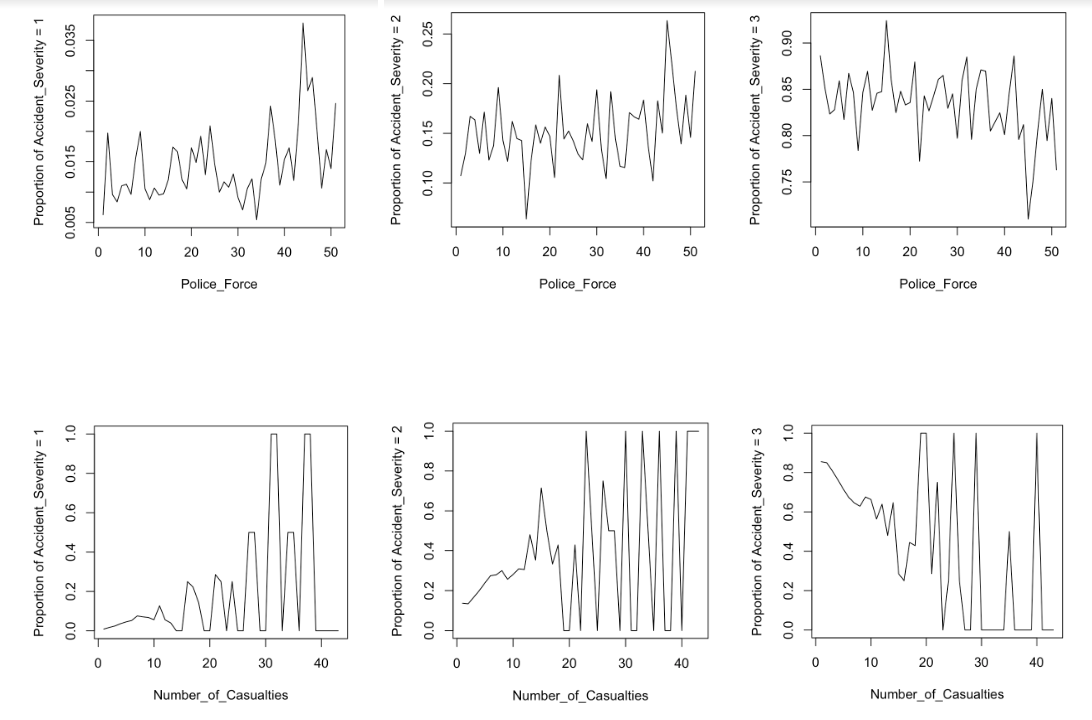
\includegraphics[width=70cm,height=7cm, scale=0.6,keepaspectratio]{severity-analysis.png}
   \end{center}

As the number of casualties and the police force increases, the probability of the accident being assigned a severity of 1 increases, and the probability of being assigned a severity of 3 decreases. The probability of being assigned a severity of 2 increases sharply at first, but then slows down. This shows that a severity of 1 is the most severe, and a severity of 3 is the least severe. \\

 \subsection{Trends}
   
   \textbf{Trend in frequency of accidents over the years:}

   \begin{center}
     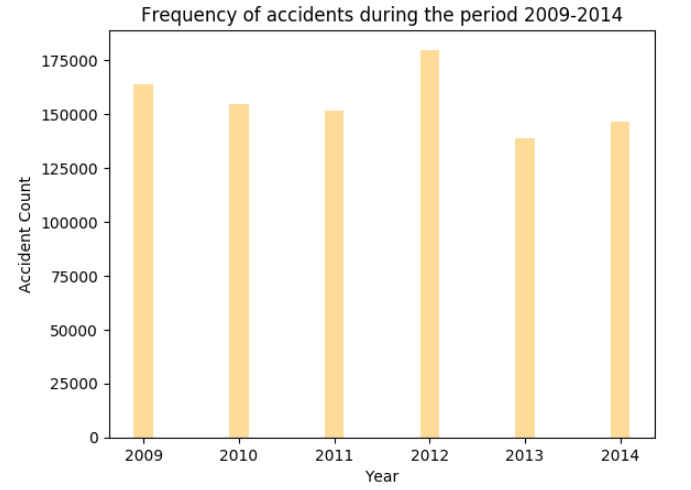
\includegraphics[width=20cm,height=5cm, scale=0.8,keepaspectratio]{counts.png}
   \end{center}

   As seen in the bar plot, the accidents seem to have very slight variations, gradually decreasing trend mostly, over the years with an exception in 2012 when the count of casualties
   shot up over 175000. However, we don't know why this abrupt increase has happened yet. \\

   The variation in the number of accidents over different hours of the day indicates that the most of the accident occur during the evening, with it's peak between 5.00pm - 6.00pm.
   This observation seems natural since more vehicles are expected after daily work hours, which usually ends around this time. \\
   
   \begin{center}
     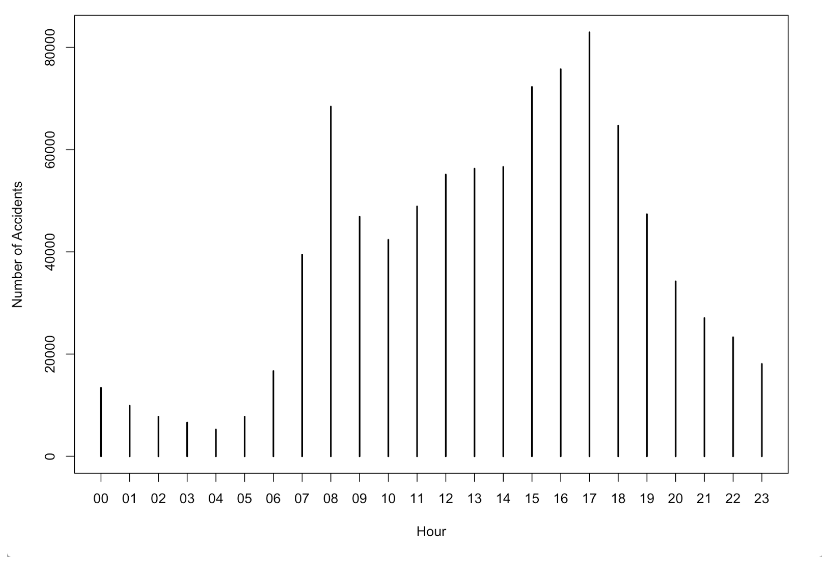
\includegraphics[width=10cm,height=6cm, scale=0.8,keepaspectratio]{hour-study.png}
   \end{center}

  Moreover, according to the plot of the frequency of accidents over days in the week, friday leads in the number of casualties. 
   
   \begin{center}
     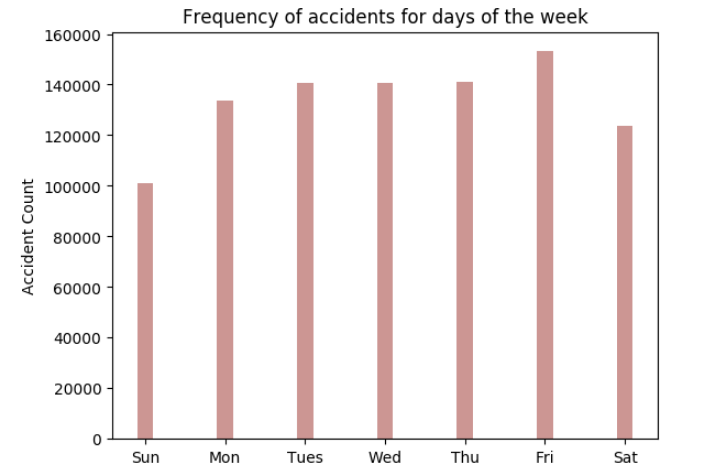
\includegraphics[width=30cm,height=5cm, scale=0.8,keepaspectratio]{day-study.png}
   \end{center}

   \textbf{Seasonal frequency of road accidents:}

   \begin{center}
     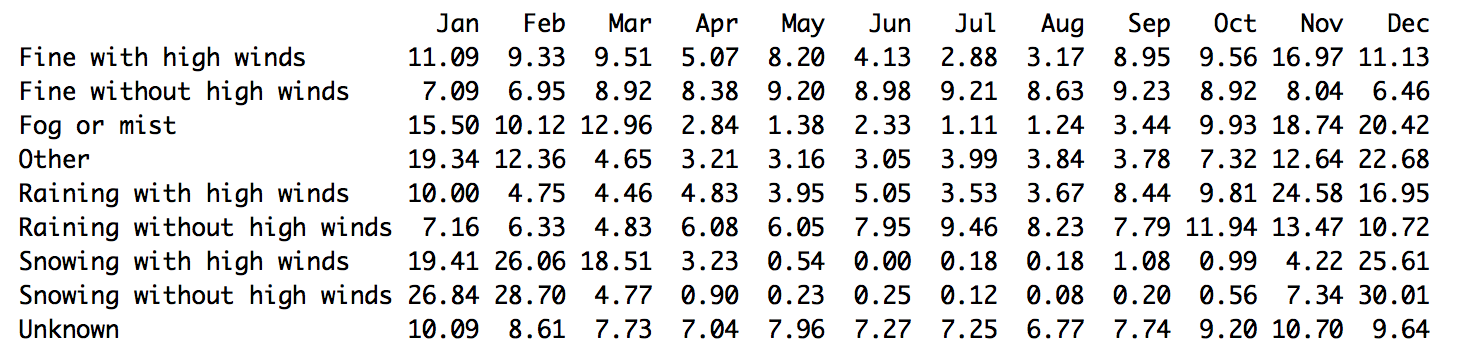
\includegraphics[width=10cm,height=7cm, scale=0.7,keepaspectratio]{seasonal-study.png}
   \end{center}

   The analysis shows that 30.1\%, 26.84\% and 28.70\% of all accidents in snowy weather occurs in December, January and February respectively. The numbers are quite high for environments with
   fog or mist, as well as snow with high winds during these months. Maybe, taking more precautions and saftey measures for the weather can bring down accidents during these months. \\

   \textbf{Trend in accident frequency with lighting conditions:}
   
   \begin{center}
     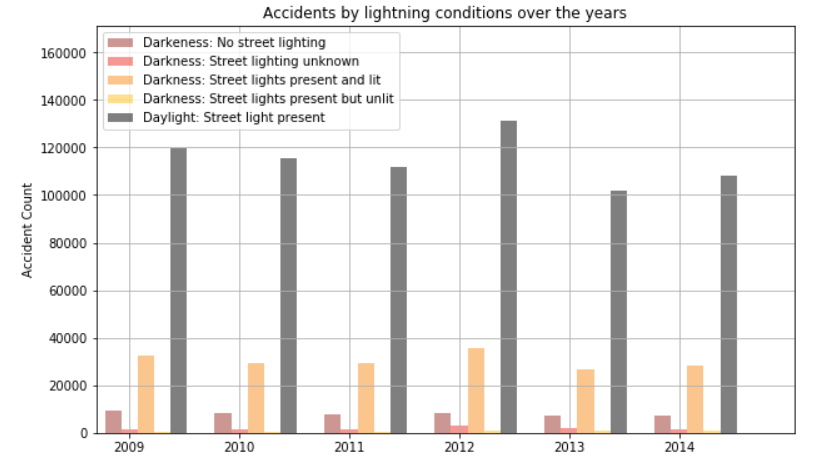
\includegraphics[width=70cm,height=7cm, scale=0.4,keepaspectratio]{lighting-study.png}
   \end{center}
   The yearly trend for accident correlation with lighting conditions hasn't shifted much over the years. As we can see, most of the accidents occur during the daylight. The number of accidents that happen during night time on roads with street light are very less compared to this. \\
   Probably, most accidents didn't occur because of insufficient lighting. In addition, the chances that lights aren't lit if they were present are highly unlikely - this could be the reason why the fourth bar is short for every year. \\

   \textbf{Trend in accident frequency with weather conditions:}
   \begin{center}
     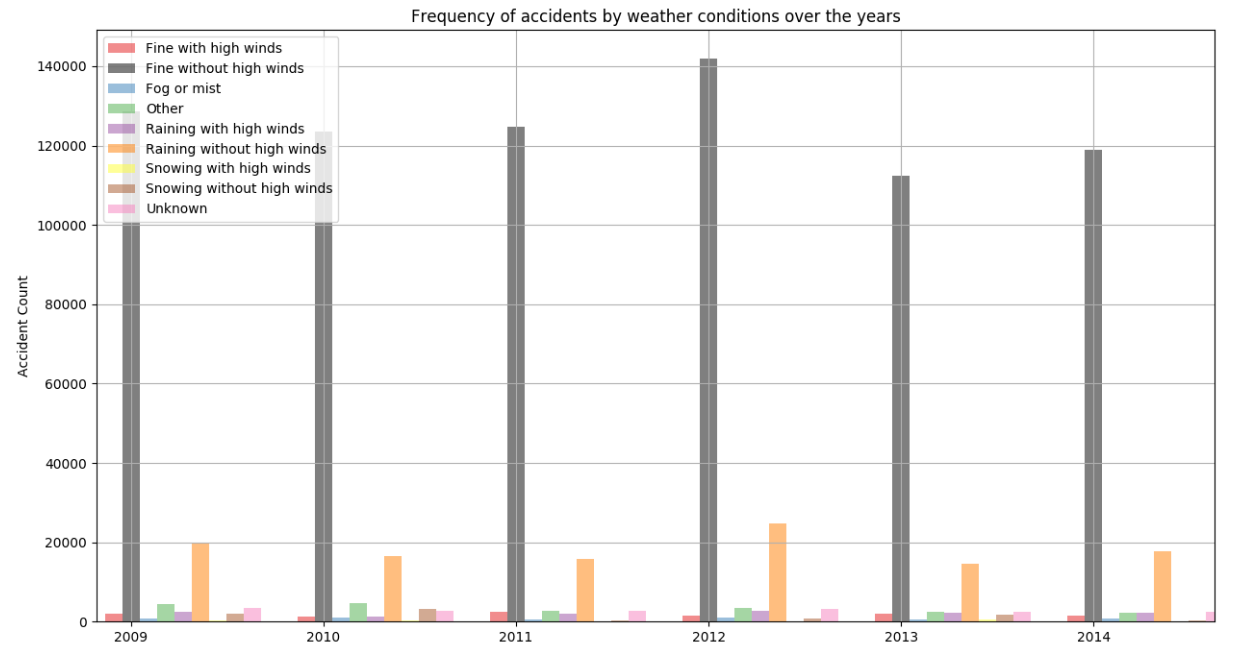
\includegraphics[width=70cm,height=7cm, scale=0.4,keepaspectratio]{weather-study.png}
   \end{center}

   After analyzing the trend in the frequency of accidents with weather conditions during the period 2009-2014, we realized that most of the accidents happen during fine weather without any wind or storm.
 Although some accidents are weather prone as disussed before, it definitely isn't the main cause of accidents. \\
   
 \section{Outliers}
 \begin{itemize}
 \item For 11 accidents, the number of casualties was over 10, but no police officer attended the scene of the accident.
 \item There are 23 accidents in the dataset for which the recorded weather is snowy, but the month is May.
 \item There is 1 accident which involved 67 vehicles.  
 \end{itemize}
   \section{Next Steps}
   
 \section{References}
 [1] \url{http://www.citymayors.com/gratis/uk\_topcities.html}
\end{document}

%%% Local Variables:
%%% mode: latex
%%% TeX-master: t
%%% End:
